\begin{multicols}{2}
   \topic{File I/O}
   \subtopic{Hard links}
   \begin{itemize}[leftmargin=*, noitemsep]
      \item Hard linking creates another file that points to the same inode number (and hence, same underlying data)
      \item If one file deleted, file data can be accessed through the other links
      \item Inode maintains a link count, file data deleted only when no further links to it
      \item You can only unlink, OS decides when to delete.
   \end{itemize}

\begin{verbatim} 
   prompt> echo hello > file
   prompt> cat file
   hello
   prompt> ln file file2
   prompt> cat file2
   hello
   
   prompt> ls -i file file2
   67158084 file
   67158084 file2
   
   prompt> rm file
   removed 'file'
   prompt> cat file2
   hello
\end{verbatim}


\subtopic{Soft links}
\begin{itemize}[leftmargin=*, noitemsep]
   \item Soft link is a file that simply stores a pointer to another filename.
\begin{verbatim}
   file
   file2 > file
\end{verbatim}
\vspace{0.5em}   

   \item If the main file is deleted, then the link points to an invalid entry: \textbf{dangling reference}.
   
\begin{verbatim}
   prompt> echo hello > file
   prompt> ln -s file file2
   prompt> cat file2
   hello
   prompt> rm file
   prompt> cat file2
   cat: file2: No such file or directory
\end{verbatim}
\end{itemize}

\columnbreak
\vspace{1em}
\textbf{What problems do we face while simple execution of an 1/O device? How to solve them? Explain in detail.}
\begin{itemize}[noitemsep]
   \item Polling status to see if device ready- wastes CPU cycles.
   \item Programmed I/O- CPU explicitly copies data to/from device.
\end{itemize}

\subtopic{Interrupts}
\begin{itemize}[noitemsep]
    \item Polling wastes CPU cycles.
    \item Instead, OS can put the process to sleep and switch to another process.\\
    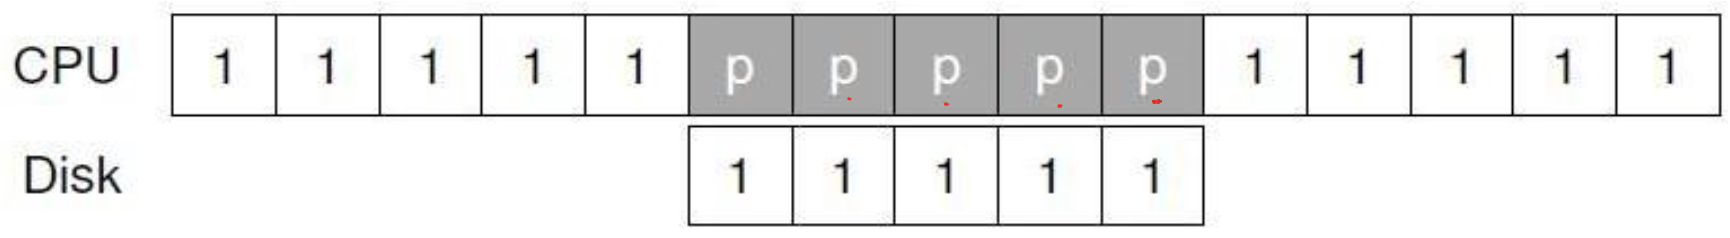
\includegraphics[width=0.95\linewidth]{figures/Interrupts1.png}
    \item When an I/O request completes, the device raises an interrupt.\\
    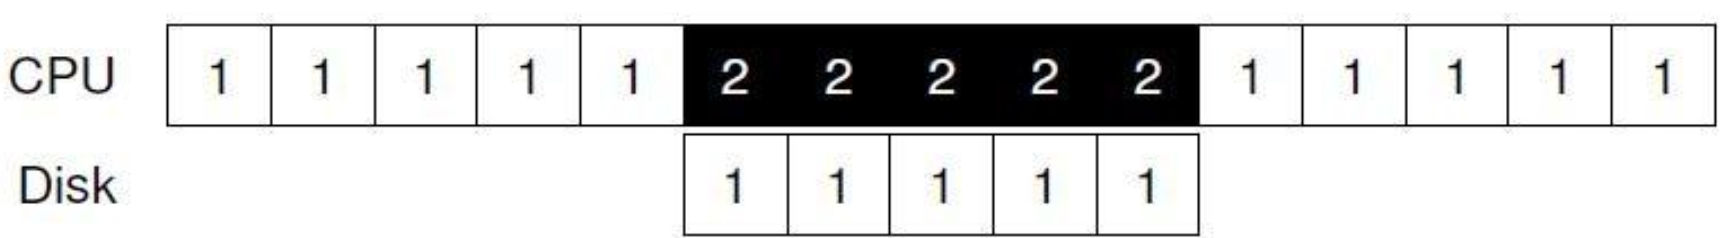
\includegraphics[width=0.95\linewidth]{figures/Interrupts2.png}
\end{itemize}


\subtopic{Direct Memory Access (DMA)}
\begin{itemize}[noitemsep]
   \item CPU cycles wasted in copying data to/from device\\
   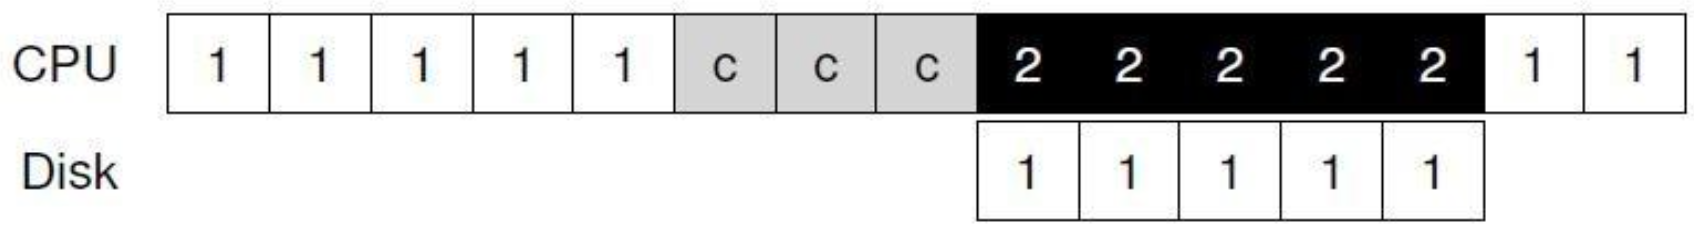
\includegraphics[width=0.95\linewidth]{figures/DMA1.png}
   \item Instead, a special piece of hardware (DMA engine) copies from main memory to device
   \begin{itemize}[noitemsep]
      \item CPU gives DMA engine the memory location of data
      \item In case of read, interrupt raised after DMA completes
      \item In case of write, disk starts writing after DMA completes
   \end{itemize}
   
   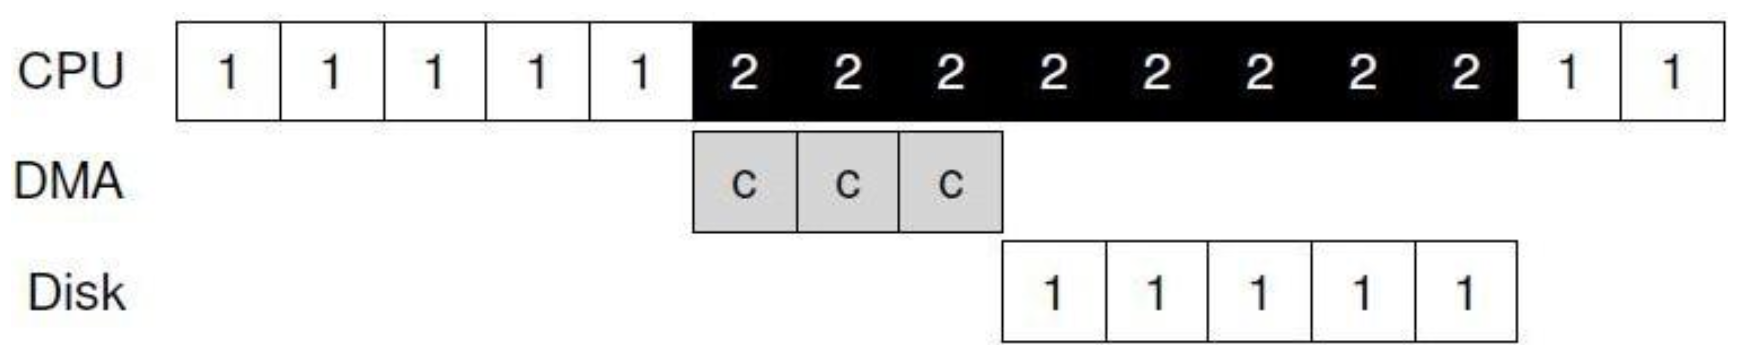
\includegraphics[width=0.95\linewidth]{figures/DMA2.png}
\end{itemize}

\end{multicols}